\documentclass[aspectratio=169]{beamer}
\usetheme{metropolis}           % Use metropolis theme
\usepackage[utf8]{inputenc}
\usepackage{graphicx}
\usepackage{eso-pic}
\usepackage{graphics}
\usepackage{tikz}
\usepackage[export]{adjustbox}
\usepackage{multicol}
\usepackage{listings}
\usepackage{helvet}
\usepackage{booktabs}
\usepackage{threeparttable}
\usepackage{xcolor}
\usepackage{hyperref}
\usepackage{soul}	% For strike-through
\usepackage{tcolorbox} % For color box



%%% Define a command to include picture in section,
%%% make section, and revert to old template
\newcommand{\sectionpic}[2]{
	\section{#1}
	\setbeamertemplate{section page}[mytheme]
}

%%% The command below allows for the text that contains Stata code
\lstset{ %
	backgroundcolor=\color{white},
	basicstyle=\tiny,
	breakatwhitespace=false,
	breaklines=true,
	captionpos=b,
	commentstyle=\color{green},
	escapeinside={\%*}{*)},
	extendedchars=true,
	frame=single,
	numbers=left,
	numbersep=5pt,
	numberstyle=\tiny\color{gray},
	rulecolor=\color{black},
	showspaces=false,
	showstringspaces=false,
	showtabs=false,
	stringstyle=\color{mauve},
	tabsize=2,
	title=\lstname,
	morekeywords={not,\},\{,preconditions,effects },
	deletekeywords={time}
}

%-----------------------------------------------
% --- Include link to last commit
\usepackage{xstring}
\usepackage{catchfile}


%-----------------------------------------------
% --- Add your information here
\title{Intro to Git and GitHub}
\author{María Reyes Retana}
\date{July 15, 2024}
\institute{Development Impact Evaluation (DIME) \newline The World Bank}
\setbeamercolor{background canvas}{bg=white} % Sets background color
\setbeamercolor{frametitle}{bg= violet, fg=white}

\newcommand{\trainingURL}[1]{{\color{blue}\url{#1}}}
\newcommand{\traininerUsername}{dime-wb-trainings}
\newcommand{\repoName}{\traininerUsername/lyrics-jul15}
\newcommand{\trainingRepoURLwithParameter}[1]{\trainingURL{https://github.com/\repoName#1}}
\newcommand{\trainingRepoURL}{\href{https://github.com/\repoName}{\trainingURL{https://github.com/\repoName}}}
\newcommand{\rootdir}{../../../}
%%% Removes "Figure X ..." from captions. It is weird that only the images with figure numbers are numbered
\setbeamertemplate{caption}{\raggedright\insertcaption\par}

% Command to set the background image
\newcommand{\setbackgroundimage}[1]{
    \usebackgroundtemplate{
    \tikz[overlay, remember picture] \node[opacity=0.9, at=(current page.center)] {\includegraphics[height=\paperheight, width=\paperwidth]{#1}};
    }
}

% ---------------------------- Preamble ends here ----------------------------

\begin{document}

\setbackgroundimage{\rootdir common-resources/img/content-slide.png} % Adjust path to your image file

\begin{frame}[plain]
	\makebox[\linewidth][c]{%
		\includegraphics[width=\paperwidth,height=\paperheight,keepaspectratio]{\rootdir common-resources/img/indonesia.png}%
	}
\end{frame}

% title slide 
{
\setbeamertemplate{background}{%
  \includegraphics[width=\paperwidth,height=\paperheight]{common-resources/img/section-slide.png} % Specific background for the title slide
}
\setbeamercolor{title}{fg=white} 
\setbeamercolor{author}{fg=white} 
\setbeamercolor{date}{fg=white} 
\setbeamercolor{institute}{fg=white} 

\begin{frame}[plain]
\titlepage 
\end{frame}
}


\begin{frame}
\frametitle{Before the session starts:}
	\begin{enumerate}
		\item Do you have a GitHub.com account? If not, go to \trainingURL{https://github.com/join} and sign up
		\item Have you shared your GitHub username with the session organizer?
		\item Have you installed GitHub Desktop? If not go to \trainingURL{https://desktop.github.com/} and download it.
		\item Have you logged in at least once on GitHub Desktop? If not open GitHub Desktop and log in using your GitHub account.
		\item Have you been invited to \trainingRepoURL{}?
		\item And have you accepted at \trainingRepoURLwithParameter{/invitations}?
	\end{enumerate}

\end{frame}

\sectionpic{Introduction}{}

\begin{frame}
\frametitle{What is Git used for?}

	\begin{columns}[c]

		\column{.60\textwidth} % Left column and width
		\begin{itemize}
			\item Git solves the \textit{Final.doc} problem
			\item <2->Common solution to the \textit{Final.doc} problem: Name all your docs like \textit{YYMMDD\_docname\_INITIALS.doc}
			\item <3->Git tracks \textit{YYMMDD} and \textit{INITIALS} for all edits  without the user having to remember it
			\item <4->That's far from everything, Git also solves:
			\begin{itemize}
				\item <4->Conflicting copy problem (DropBox etc.)
				\item <4->I can't re-produce my Baseline report problem
				\item <4->Who wrote this code 4 years ago and why?
				\item <4->And much much more...
			\end{itemize}
		\end{itemize}

		\column{.40\textwidth} % Right column and width
		\begin{figure}
			\centering
			\includegraphics[width=1\linewidth]{img/finaldoc_cartoon}
			\label{fig:finaldoccartoon}
		\end{figure}

	\end{columns}
\end{frame}


\begin{frame}
	\frametitle{What is Git, GitHub and GitHub Desktop?}
	\begin{figure}
		\centering
		\includegraphics[width=0.7\linewidth]{img/git_github_gitclient_git}
		\label{fig:gitgithubgitclient_git}
	\end{figure}
\end{frame}

\begin{frame}
	\frametitle{What is Git, GitHub and GitHub Desktop?}
	\begin{figure}
		\centering
		\includegraphics[width=0.7\linewidth]{img/git_github_gitclient_github}
		\label{fig:gitgithubgitclient_github}
	\end{figure}
\end{frame}

\begin{frame}
	\frametitle{What is Git, GitHub and GitHub Desktop?}
	\begin{figure}
		\centering
		\includegraphics[width=0.7\linewidth]{img/git_github_gitclient_gitclient}
		\label{fig:gitgithubgitclient_gitclient}
	\end{figure}
\end{frame}

\begin{frame}
\frametitle{What will we learn?}

	In \textbf{An intro to Git and GitHub - Contributor Role} you will learn to:

	\begin{itemize}
		\item Explore the history of a project folder in GitHub and see what different team members are currently working on
		\item Download a project folder from GitHub so you can work on it
		\item Create a space in the project folder where you can make your edits
		\item Make edits and share those versions with your team. When you are ready, request that your edits are included in the main version
	\end{itemize}

\end{frame}


\begin{frame}
\frametitle{MVO}

	\hspace*{2.5cm}\Large{Three Git concepts needed to do this:}

	\begin{itemize}
		\setlength{\itemindent}{3cm}
		\Large{\item Clone}
		\Large{\item Commit}
		\Large{\item Branch}
	\end{itemize}

\end{frame}


\begin{frame}
\frametitle{Code free training!}

	\begin{columns}[c]

		\column{.15\textwidth} % Left column and width

		\column{.70\textwidth} % Left column and width
		\textbf{No code today!}

		\vspace{.5cm}

		We will not work with code today.

		\vspace{.25cm}

		Code tends to distract people if, for example, they see a command they do not understand.

		\vspace{.25cm}

		Instead we will work with lyrics in .txt files that works exactly the same as code files in Git.

		\column{.15\textwidth} % Left column and width

	\end{columns}
\end{frame}

\begin{frame}
\frametitle{How to browse GitHub.Com}

	Your project folder is called a \textbf{repository} in Git, often \textbf{repo} for short.
	When you enter \trainingRepoURL{} you get to what we will call the \textbf{repository landing page}.

	\vspace{.5cm}

	\begin{columns}[T]

		\column{.55\textwidth} % Left column and width
		Go from \textbf{GitHub.com} to \textbf{repo}
		\begin{enumerate}
			\item From anywhere on \trainingURL{github.com} click the \textit{octocat} icon in the top left corner.
			\item In the menu to your left you see the repositories you are invited to
			\item Click any repo to get to the landing page of that repo.
		\end{enumerate}

		\column{.45\textwidth} % Left column and width
		Go from \textbf{repo} to \textbf{landing page}
		\begin{enumerate}
			\item Click the repo name in {\color{blue}\url{\repoName}} at the top of any page within the repo
		\end{enumerate}

	\end{columns}
\end{frame}

\sectionpic{Clone}{}

\begin{frame}
\frametitle{What is cloning?}

	Cloning is similar to downloading a \textbf{repository} to your computer.

	\vspace{.5cm}

	The difference between cloning and downloading is that \textbf{when Git clones a repository it remembers where you downloaded it from}. This is necessary so that Git knows where send any edits you make to the files when sharing them with your team.

\end{frame}

\begin{frame}
\frametitle{How do I clone a repository from GitHub?}

	\begin{columns}[c]

		\column{.70\textwidth} % Left column and width
		How to clone a repository:
		\begin{enumerate}
			\item Go to the \textbf{landing page} of \trainingRepoURL{}
			\item Click the green \textit{Code} button (see image)
			\item Click \textit{Open with GitHub Desktop}
			\item Select where on your computer to clone the repository. Do \textbf{NOT} clone in a shared folder, like a network drive or in DropBox. Create a \textit{GitHub} folder in non-synced location and clone there. Read more about this in our guide {\color{blue}\href{https://github.com/worldbank/dime-github-trainings/blob/master/GitHub-resources/DIME-GitHub-Guides/clone-location.md}{here}}.
		\end{enumerate}

		\column{.30\textwidth} % Left column and width
		\begin{figure}
			\centering
			\includegraphics[width=1\linewidth]{img/clonedownload_button}
			\label{fig:clonedownloadbutton}
		\end{figure}

	\end{columns}

\end{frame}


\begin{frame}
\frametitle{Explore the clone}

	\begin{columns}[c]

		\column{.20\textwidth} % Left column and width

		\column{.60\textwidth} % Left column and width
		\textbf{Explore the clone!}

		\vspace{.5cm}

		Compare the files and folders you cloned to your computer with those in the repository on \trainingRepoURL{}

		\column{.20\textwidth} % Left column and width

	\end{columns}

\end{frame}

\sectionpic{Collaboration on a repository}{}

\begin{frame}
\frametitle{Collaboration needs two more concepts}

	\center{In order to collaborate on a repository we need to introduce two topics:}

	\vspace{1cm}

	\begin{columns}[c]

		\column{.30\textwidth} % Left column and width
		\center{\huge{\textbf{Commits}}}

		\column{.30\textwidth} % Left column and width
		\center{\huge{\textbf{Branches}}}

	\end{columns}

	\vspace{2cm}

\end{frame}

\sectionpic{Commit}{}

\begin{frame}
\frametitle{What is a version in version control?}

	\begin{columns}[c]

		\column{.50\textwidth}
		First look at how version control works in another software you might be familiar with.

		\vspace{.5cm}

		In DropBox each saved version of a file is saved to the version history. This is the only way to do it automatically, but are all these versions meaningful differences?

		\column{.50\textwidth}
		\begin{figure}
			\centering
			\includegraphics[width=1\linewidth]{img/dropbox_versioncontrol}
			\label{fig:dropboxversioncontrol}
		\end{figure}

	\end{columns}


\end{frame}

\begin{frame}
\frametitle{What is a commit?}

	Instead of having a list of each saved version of a file, in Git we use \textbf{commits to indicate what is each meaningful difference between two versions of our project folder}.

	\vspace{.25cm}

	Each commit is a snapshot of all files in the project folder and lists how that snapshot differs from the previous snapshot (the previous commit).

	\vspace{.25cm}

	Each commit has a time stamp and tracks who did the commit. This is very similar to the \textit{YYMMDD\_docname\_INITIALS.doc} solution to the \textit{Final.doc} problem.

\end{frame}

\begin{frame}
\frametitle{How to make a commit}

	We need to introduce \textit{branches} before we can all commit to the same repository, so for now, let me show you how to make a commit:

	\begin{enumerate}
		\item I add a new lyrics .txt file in the clone
		\item I use GitHub desktop to commit the new file to the repository
		\item Can you see the new file on your computer?
		\item Can you see it if you sync in GitHub Desktop?
	\end{enumerate}

\end{frame}


\begin{frame}
\frametitle{Exploring commits}

	Now that we know what a commit is, we can explore how the \trainingRepoURL{} repository was created.

	\vspace{.25cm}

	We will see a list of commits, that at first sight is similar to the the version history in DropBox, but \textbf{in Git the version list is more meaningful, as it is a list of only meaningful differences}.

	\vspace{.25cm}

	\begin{itemize}
		\item \trainingRepoURLwithParameter{/commits}
		\item This list can also be found in GitHub Desktop in the \textit{History} tab
	\end{itemize}

\end{frame}

\sectionpic{Branches}{}

\begin{frame}
\frametitle{Introducing branches}

	\begin{columns}[c]

		\column{.60\textwidth}
		\textbf{Branches is the "killer feature" of Git}. This is where Git becomes really powerful as a collaboration tool and not just as version control.

		\vspace{.25cm}

		Branches allows you to \textbf{create a copy of the code where you can experiment}, if you like the result, \textbf{you can very easily merge your experiment with the main version of your code}.

		\vspace{.25cm}

		This non-linear version control is much more similar to how we actually work than the strictly linear version control in, for example, DropBox

		\column{.40\textwidth}
		\begin{figure}
			\centering
			\includegraphics[width=1\linewidth]{img/branches}
			\label{fig:branches}
		\end{figure}

	\end{columns}

\end{frame}

\begin{frame}
\frametitle{Looking at branches}


	\textbf{One more way to explore the repository:}
	\begin{itemize}
		\item Linear progression -$>$ \trainingRepoURLwithParameter{/commits}  
		\item Non-linear progression -$>$ \trainingRepoURLwithParameter{/network} 
	\end{itemize}

	\vspace{.05cm}

	\textbf{Exploring branches}
	\begin{itemize}
		\item You can change branch in \textit{/commits}. What happens then?
		\item Go to the landing page, what happens if you change the branch here?
		\item Which version is in the clone on your computer? They are all actually in your clone, but only one is shown - \textbf{checked out} - at the time
		\item What happens to the files on your computer when you check out another branch in GitHub Desktop?
	\end{itemize}

\end{frame}

\begin{frame}
\frametitle{Working with branches}

	A typical Git work flow involves multiple branches and there are tools in GitHub to makes that work flow easy, but that is not within today's scope. Although, what you should know after this training is only how to create your own branch and how to commit to it.

	\textbf{Create a branch:}
	\begin{itemize}
		\item Go to \trainingRepoURL{} and click the button where it says \textit{Branch: main}.
		\item Write your name in the field and click \textit{Create branch: your\_name}. Make sure it says \textit{from 'main'}.
		\item See how the button now says \textit{Branch: your\_name}
	\end{itemize}

\end{frame}

\sectionpic{Combining Commit \& Branch}{}

\begin{frame}
\frametitle{Now it is time to collaborate}

\textbf{Now it is time for you to collaborate:}
\begin{enumerate}
	\item Make sure your branch is checked out in GitHub Desktop.
	\item Open a text editor. It could be \textit{Notepad} if you are using Windows, \textit{TextEdit} if you are using Mac, or any other code editor like \textit{Atom}, or \textit{Notepad++} etc.
	\item Google the lyrics of your favorite song, and copy the lyrics to a new file in the text editor you just opened
	\item Save the lyrics in your local clone according to these instructions:
	\begin{itemize}
		\item Save the file in \textit{.txt} format (Especially Mac users, this is not always the default)
		\item Name the file after the title of the song
		\item Save it in the appropriate genre folder (create a new genre folder if needed)
	\end{itemize}
\end{enumerate}

\end{frame}

\begin{frame}
\frametitle{Do your first commit}

\begin{columns}[c]

\column{.60\textwidth} % Left column and width

\begin{enumerate}
	\item Open the changes tab in GitHub Desktop
	\item GitHub Desktop tracks your clone and has noticed that you changed something in it
	\item Then you need to do the three steps required to commit a file to the repository:
	\begin{enumerate}
		\item Make sure the file you want to add is checked
		\item Write a commit message
		\item Click \textit{Commit to your\_name} - check out your branch if it says \textit{main}
		\item Click the sync button
	\end{enumerate}
\end{enumerate}

\column{.40\textwidth} % Left column and width
\begin{figure}
	\centering
	\includegraphics[width=1\linewidth]{img/desktop_changes}
	\label{fig:desktopchanges}
\end{figure}

\vspace{-1cm}

\begin{figure}
	\centering
	\includegraphics[width=1\linewidth]{img/desktop_commit}
	\label{fig:desktop_commit}
\end{figure}

\end{columns}

\end{frame}

\begin{frame}
\frametitle{Check your contribution}

	\textbf{Check your commit on GitHub:}
	\begin{itemize}
		\item Can you find your commit at: \trainingRepoURLwithParameter{/network}
		\item Can you find your commit at: \trainingRepoURLwithParameter{/commits}
	\end{itemize}

	If you cannot see your commit, make sure that you are looking in the correct branch.

\end{frame}

\begin{frame}
\frametitle{Pull Requests}

	A feature related to branches is a \textbf{pull request}.
	When the edits you have done in your branch
	are ready to be merged with the main version of the code,
	you make a pull request, i.e. you are requesting that
	your edits are pulled into the main branch.


	A pull request can be made either by the person that edited the branch or the repo maintainer.

	It is common in GitHub repositories that only the repo maintainer has access to the main branch, and pull requests are then the only way to contribute to the main branch.


\end{frame}

\begin{frame}
\frametitle{Merge your contribution}

	\textbf{To make a pull request for your branch:}
	\begin{itemize}
		\item Go to \trainingRepoURLwithParameter{/pulls} and click \textit{New pull request}
		\item Make sure that the \textit{main} branch is selected as the \textit{base:} branch, and then select your branch as the \textit{compare:} branch
		\item Scroll down to check the edits you are requesting to be pulled in to the main branch. If it looks ok, then click \textit{Create pull request}
		\item Then you have the chance to add more instructions if you want, then click \textit{Create pull request} again
	\end{itemize}
\end{frame}

\begin{frame}
\frametitle{Merge your contribution}

Can you see your lyrics file in the main branch now? Why not?

\vspace{.5cm}

Your contribution will not be included until the branch is merged. We have more trainings on the details of merging branches but for now, this is all you need to know:

	\begin{itemize}
		\item Always have someone to review your PR before merging it
		\item Always delete your branch after it is merged - you can always recreate a new branch with the same name if you want
	\end{itemize}

\end{frame}



\begin{frame}
\frametitle{What have we learned?}

	In \textbf{An intro to Git and GitHub - Contributor Role} you have learned to:

	\begin{itemize}
		\item Explore the history of a project folder in GitHub and see what different team members are currently working on
		\item Download a project folder from GitHub so you can work on it
		\item Create a space in the project folder where you can make your edits
		\item Make edits and share those versions with your team. When you are ready, request that your edits are included in the main version
	\end{itemize}

\end{frame}

\begin{frame}
\frametitle{What have we learned?}

	In \textbf{An intro to Git and GitHub - Contributor Role} you have learned to:

	\begin{itemize}
		\item Explore the history of \textbf{repository} and see what different team members are currently working on
		\item \textbf{Clone} a \textbf{repository} so you can work on it
		\item Create a \textbf{branch} in the \textbf{repository} where you can make your edits
		\item Make edits and share \textbf{commits} with your team. When you are ready, make a \textbf{pull request} to the \textbf{main branch}
	\end{itemize}
\end{frame}

\sectionpic{Setting up a Good Workflow}{}

\begin{frame}{Importance of structuring data work}
	
		\begin{itemize}
            \item Research projects are often long, have multiple team members, and involve many different data-sets

            \vspace{.2cm}
            \item During the typical project lifetime, many team members will make crucial contributions -- and it is likely that not all of them were part of the initial planning

            \vspace{.2cm}
		  	\item Therefore, it is important to both organize all of our data work and set up an effective "inter-generational" data work communication
		  	
		  	\vspace{.2cm}
		  	\item This is best done before any code is written -- however, edits and additions will be required during the course of a project
        \end{itemize}
	
\end{frame}

\begin{frame}{Importance of structuring data work}
	
		\begin{itemize}
            \item Taking time for these tasks at the beginning of project will save time over the project's full life-cycle
            \vspace{.2cm}
            \item This helps senior team members to explain tasks they delegate, as well as helping junior team members to confirm and communicate their understanding of those tasks to their supervisors
            \vspace{.2cm}
            \item Having a good structure from the beginning makes it easier to collaborate and save valuable time on communicating and explaining the different moving parts of a project
              \vspace{.2cm}
            \item Will help to make your work clearer and less error-prone. If errors or changes are required, it will be easier to implement them. 
        \end{itemize}
	
\end{frame}

\begin{frame}{Key takeaways}

	In this part of the session, we will cover
    \begin{itemize}
            \item \texttt{GitHub Repository}: Start your project by including version control in GitHub to improve collaboration.
	    \item \texttt{Folder structure}: Organizing your project folder for effective collaboration.
        \item \texttt{Main scripts}: One script that run all project code.
        \item \texttt{Documentation}: README file containing relevant project information, decisions, instructions, etc.
  \end{itemize}
   Organizing your data work using these principles will make your research more effective, efficient, and reproducible!

\end{frame}


\begin{frame}
\frametitle{Structure of a good workflow}
\begin{figure}[h!]
    \centering
    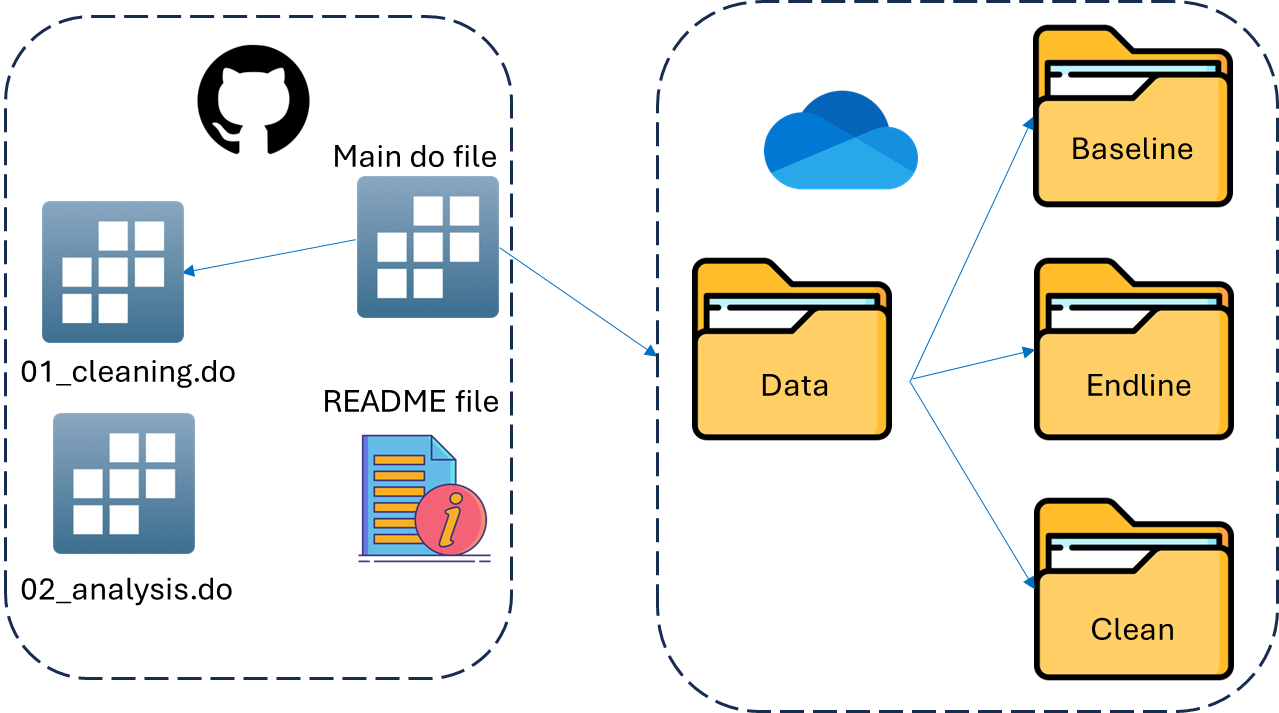
\includegraphics[width=0.8\linewidth]{img/structure_flow.png}
    \caption{Example of a Good Workflow}
\end{figure}
\end{frame}

\begin{frame}
\frametitle{GitHub: repository creation}
\begin{itemize}
    \item \textbf{Steps for Repository Creation}
    \begin{enumerate}
        \item Go to \href{https://github.com/}{GitHub} and log in to your account.
        \item Click on the "New" button to create a new repository.
        \item Enter a name for your repository.
        \item Set the repository visibility to private if necessary.
        \item Click "Create repository".
    \end{enumerate}
    \item Note: In this case, the repository has already been created, as it normally will in a regular project. This demonstration is for reference.
\end{itemize}
\end{frame}

\begin{frame}
\frametitle{Hands-on: cloning the mock project}
Once your project has a repository. 
\begin{itemize}
    \item \textbf{Clone the repository}
    \begin{enumerate}
        \item Go to the GitHub repository: \texttt{https://github.com/dime-wb-trainings/GitHub-MockProject}.
        \item Click on the green "Code" button and select "Open with GitHub Desktop".
        \item Follow the prompts to clone the repository to your local machine.
    \end{enumerate}
    \end{itemize}
\end{frame}

\begin{frame}
\frametitle{Hands-on: create a branch in the mock project}
Once you have the repository on your computer:
\begin{itemize}
    \item \textbf{Create a branch}
    \begin{enumerate}
        \item As we will be working collaboratively, create a branch named "workflow\_" followed by your initials.
        \item Switch to that branch to start making changes to the project.
    \end{enumerate}
    \item When working on a real project, follow the principle: \textbf{branch often, merge often}. In practice:
    \begin{itemize}
        \item Create a branch for each task.
        \item After completing the task, merge the branch back to the main branch by creating a Pull Request (PR).
        \item Repeat this process for subsequent tasks to ensure smooth and collaborative development.
    \end{itemize}
\end{itemize}
\end{frame}

\begin{frame}{Folder structure}

	\begin{itemize}
	    \item At the beginning of a research project, organize your data work into a folder structure that is easy to follow
    	\item Think about all the sources and rounds of data that your project is anticipated to have
    	\item Have one separate sub-folder for each source of data, and keep sub-folders for each data source as similar as possible
    	\item Avoid creating individual folders in an ad-hoc manner as the need arises - be methodological
    	
	\end{itemize}

\end{frame}

\begin{frame}
\frametitle{Hands-on: folder structure}
\begin{itemize}
    \item Download the mock data from the provided link.
    \item Save the data files in the \texttt{data/} folder on your local machine.
    \item Arrange the folder structure intuitively:
    \begin{itemize}
        \item \texttt{code/} - Folder for all Stata scripts.
        \item \texttt{data/} - Folder for data files (not tracked by Git).
        \item \texttt{outputs/} - Folder for your outputs, if relevant.
        \item \texttt{README.md} - Project documentation.
        \item \texttt{.gitignore} - Specify files and folders to ignore in Git.
    \end{itemize}
\end{itemize}
\end{frame}

\begin{frame}{Main script}
	
	\begin{itemize}	
       	\item The most important purpose of the \textbf{main script} is to have one script that
       	runs all other scripts in the intended order
       	\item It should never be required that that a human needs to know in which order scripts need to run in order for the project code to execute correctly
       	\item Having a text-file or file-naming convention that communicate the run order is marginally better, but still error prone
       	\item A main file that automatically run all files in correct order is the best practice and a requirement in DIME Analytics' reproducibility verification -- we call this "One-click Reproducibility"
    \end{itemize}
\end{frame}

\begin{frame}{Main script - additional benefits}

	\begin{itemize}
		
		\vspace{.2cm}
		\item The main script becomes an ordered table of contents for all data work 
		\vspace{.25cm}
  	
		\item Specify settings and other requirements in one place -- such as:
		\begin{itemize}
			\item Check and install software packages needed in the project code
			\item Set any setting needed to make random processes reproducible
			\item Set project-wide variables such as conversion rates or list of control variables
		\end{itemize}	

        \vspace{.25cm}

        \item \textbf{Collaboration} 
        \begin{itemize}
			\item Use globals (Stata) dynamically set root paths.
            \item Other can set-up the project on their computer by just setting the root paths -- useful for collaboration and essential for one-click reproducibility.
		\end{itemize}	

	\end{itemize}
\end{frame}



\begin{frame}[fragile]{Hands-on: main script setup}
		\begin{itemize}
    \item \textbf{Create a \texttt{main.do} basic}
    \begin{itemize}
        \item Open a new Stata do-file and save it as \texttt{main.do} in the \texttt{code/} folder. (in this exercise the main.do is already in your cloned folder, but is empty)
        \item Set the global paths and the instructions to run the codes for your project in \texttt{main.do} (level one):
         \end{itemize}
\end{itemize}
		\begingroup
		\tiny
		\begin{verbatim}
			
                * Main do file for GitHub-MockProject
   
                * Set global paths (user should change accordingly)
                
                global data-path "path/to/your/data/folder"

                global code-path "path/to/your/code/folder"

                * Run Scripts 

                do "${code-path}/01-cleaning-script.do"
		
		\end{verbatim}
		\endgroup
	\end{frame}

 \begin{frame}[fragile]{Hands-on: main script setup}
		\begin{itemize}
    \item \textbf{Create a \texttt{main.do} advanced}
    \begin{itemize}
        \item For a more advanced way to set up your global paths you can do the following. 
        \item If plenty of people are collaborating this could help not to change the file paths every time you download the main file. 
         \end{itemize}
\end{itemize}
		\begingroup
		\tiny
		\begin{verbatim}
			
                * Main do file for GitHub-MockProject
   
                * Set global paths (user should change accordingly)
                
                * Research Assistant folder paths
                if "`c(username)'" == "ResearchAssistant" {
                global data-path "path/to/your/data/folder"
                global code-path "path/to/your/code/folder"
               }

                * Run Scripts 

                do "${code-path}/01-cleaning-script.do"
		
		\end{verbatim}
		\endgroup
	\end{frame}

 \begin{frame}
\frametitle{README file}
\begin{itemize}
    \item \textbf{Quick Project Overview}
    \begin{itemize}
        \item Provides a summary of the project's purpose and objectives.
        \item Helps new contributors quickly understand the project's scope and goals.
    \end{itemize}
    \item \textbf{Setup Instructions}
    \begin{itemize}
        \item Guides new team members on how to set up the project locally.
        \item Lists necessary software, dependencies, and installation steps.
    \end{itemize}
    \item \textbf{Documentation of Key Decisions}
    \begin{itemize}
        \item Records important decisions made during the project.
        \item Provides context for the project's development and structure.
    \end{itemize}
    \item \textbf{Instructions for Use}
    \begin{itemize}
        \item Details how to run and use the project.
        \item Includes examples and explanations of key functionalities.
    \end{itemize}
    \item \textbf{Improves Collaboration}
    \begin{itemize}
        \item Facilitates onboarding of new team members.
        \item Ensures consistency and clarity in communication.
    \end{itemize}
\end{itemize}
\end{frame}


\begin{frame}
\frametitle{Hands-on: README File}
\begin{itemize}
    \item \textbf{Add a \texttt{README.md}}
    \begin{itemize}
        \item Provide an overview of the project.
        \item Include instructions on how to set up the project locally.
        \item Note: The \texttt{README.md} is already there, but it is just a skeleton; participants should complete it.
        \item Example of a good README can be found here: 
        \href{https://github.com/social-science-data-editors/template_README/blob/release-candidate/templates/README.md}{Template README.md}
    \end{itemize}
\end{itemize}
\end{frame}

\begin{frame}
\frametitle{Other Elements: .gitignore}
\begin{itemize}
     \item \textbf{Usefulness of \texttt{.gitignore} file}
        \begin{itemize}
            \item Prevents sensitive or unnecessary files from being tracked in the repository.
            \item Keeps the repository clean and focused on relevant files.
            \item Avoids conflicts by ignoring files that are specific to individual environments.
            \item By default, our template should include data and `.xlsx` files in `.gitignore` for several reasons:
            \begin{itemize}
                \item Binary files are not well tracked in GitHub.
                \item Ensures privacy and data security by not including sensitive data files.
            \end{itemize}
        \end{itemize}
    \item \textbf{Explore \texttt{.gitignore} file}
    \begin{itemize}
        \item Note: The \texttt{.gitignore} file is already there, you don't need to create it, but in a project, you might.
        \end{itemize}
   
\end{itemize}
\end{frame}


\begin{frame}{Useful links: GitHub}
	\begin{itemize}
		\item All DIME Analytics GitHub trainings: \trainingURL{https://osf.io/e54gy/}
		\item Other DIME Analytics GitHub resources: \trainingURL{https://github.com/worldbank/dime-github-trainings}. For example:
		\begin{itemize}
			\item DIME Analytics GitHub Templates (for example .gitignore): \trainingURL{https://github.com/worldbank/dime-github-trainings/tree/master/GitHub-resources/DIME-GitHub-Templates}
		\end{itemize}
		\item Markdown cheat sheet (how to format text on GitHub.com):  \trainingURL{https://www.markdownguide.org/cheat-sheet/}
	\end{itemize}
\end{frame}

\begin{frame}{Useful links: Workflow}
	\begin{itemize}
		\item Template Main do file: \trainingURL{https://github.com/worldbank/dime-data-handbook/blob/main/code/box-2-4-stata-master-dofile.do}
		\item Template README \trainingURL{https://github.com/social-science-data-editors/template_README/blob/release-candidate/templates/README.md}. For example:
	\end{itemize}
\end{frame}

\end{document}
